\lab{Algorithm}{The Knapsack Problem}{The Knapsack Problem}
\label{Ch:Knapsack}

\objective{This section teaches about NP-hard problems using the knapsack problem as an example.}

\section*{The Knapsack Problem}

%Lab \ref{Knapsack}

\begin{figure}[H]
%\begin{center}
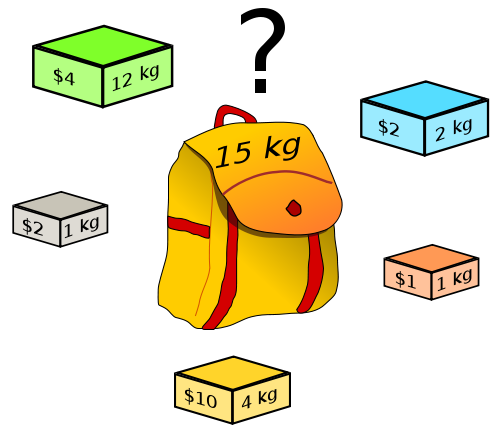
\includegraphics[scale = .3]{Knapsack.png}
\caption{Visualization of the Knapsack problem TODO: Make a picture similar to this}
%\end{center}
\end{figure}

The two dimensional Knapsack problem is you are given a knapsack that can only hold a certain weight. You have a plethera of items that have value and weight. The goal is to find the combination of items that have the most value with out exceeding the weight. Will focus on the 0/1 knapsack problem, which states that each item must be put in entirely or not at all.

A three dimensional version the items would have volume and the knapsack can only hold an certain volume as well as weight. 

This problem is has many different applications for disecion making in a wide variety of fields. Two examples are finding the least wasteful way to cut raw materials and the selection of capital investments and financial portfolios. In resource allocation wherever there are financial constraints this problem offten appears.  

\begin{problem}
Write a function that solves the Knapsack problem by testing all the combination and choosing the one with the most value that meets the weight constraint. Only test it up to 15 objects.
\end{problem}

This way finds the optimal solution, but there is a problem. Given $n$ objects the number of combinations is $2^n$. The complecity of the problem grows fast. For example, if you had 50 items, it would take more than 10 years to compute the optimal solution. For all the following timing problems let your items have vaules between 1 and 100 and the weights between 1 and $\frac{Capacity}{10}$.

\begin{problem}
Time the Knapsack problem for $11-20$ items with a carrying capacity of $10,000$. Plot the times. What is the complexity of the algorithm for increasing the number of items?
\end{problem}

\begin{problem}
Time that algorithm for the carrying capacities $10,000-90,000$ every mutiple of $10,000$ with $15$ items. Plot the times. What is the complexity of the algorithm for increasing the weight?
\end{problem}

\section*{NP-Hard}

Any problem that is not polynomial time is know as NP-hard. The Knapsack Problem is a NP-hard problem. Using the branch and bound approach we can find the optimal solution in psuedo-polynomial time.

\section*{Branch and Bound method}
We calculate the optimal solution using only the first i items for weights 0 through W (where W is the max weight the knapsack can hold)

We do this by intializing 0th row to being empty.
For i$>$0 row we go through j (being the weight) from 1 thorugh W. If the ith element's weight is more than j then the optimal combination is the same as it was for i-1. If ith element's weight is less than j, then we compare the combination at i-1 at wieght j to the combination i-1 at the weight j-the ith element weight plus the ith element. Whichever one has a higher value is the optimal combination using the first ith elements less than or equal to the wieght of j. You continue this until you have done all n elements. The combination using n items with a weight of W is guaranteed to be the optimal combination.

This only does $W*n$ checks, so it is a lot faster. This works by eliminating combinations that could not be the optimal solution

\begin{problem}
Write a function that solves the Knapsack problem using the branch and bound method.
\end{problem}

\begin{problem}
Time the Knapsack problem for $11-20$ items with a carrying capacity of $10,000$. Plot the times. What is the complexity of the algorithm for increasing the number of items? For the items use the same specifications as in the previous timing problems.
\end{problem}

\begin{problem}
Time that algorithm for the carrying capacities $10,000-90,000$ every mutiple of $10,000$ with $15$ items. Plot the times. What is the complexity of the algorithm for increasing the weight?
\end{problem}
